% !TEX program = xelatex
% ===================================================================
%  مقاله: بررسی عددی تقویت گسیل خودبه‌خودی و راندمان تابشی گسیل‌گر
%  کوانتومی در مجاورت نانومیله پلاسمونی طلا با روش 3D-FDTD
%  ---------------------------------------------------------------
%  کامپایل: xelatex main → biber main → xelatex main → xelatex main
%  یا به‌سادگی:  latexmk -xelatex main.tex
%
%  این فایل، متن موجود مقاله را با بخش‌های نوِ پیش‌نویس ادغام می‌کند:
%    - draft/abstract_and_title.md      → عنوان، چکیده، کلیدواژه‌ها
%    - draft/section1_intro_addition.md → دو پاراگراف پایانی بخش ۱
%    - draft/section2.md               → بخش ۲ (کاملاً نو)
%    - draft/section45_and_conclusion.md → زیربخش ۴.۵ + نتیجه‌گیری
%  نگاشت بخش‌ها در evidence/integration_plan.md آمده است.
% ===================================================================
\documentclass[12pt,a4paper]{article}

% --- ریاضیات (پیش از xepersian بارگذاری شود) -----------------------
\usepackage{amsmath}
\usepackage{amssymb}

% --- گرافیک، جدول، پیوند ------------------------------------------
\usepackage{graphicx}
\usepackage{booktabs}
\usepackage{caption}
\usepackage[margin=2.5cm]{geometry}
\usepackage{xcolor}

% --- کتاب‌نامه: biblatex با سبک عددی ------------------------------
\usepackage[
  backend=biber,
  style=numeric-comp,
  sorting=none,          % ترتیب ظهور در متن
  maxbibnames=99,
  giveninits=true,
  doi=true,
  isbn=false,
  url=false
]{biblatex}
\addbibresource{references.bib}

% --- پیوندها (پیش از xepersian) -----------------------------------
\usepackage{hyperref}
\hypersetup{
  colorlinks = true,
  linkcolor  = black,
  citecolor  = blue!55!black,
  urlcolor   = blue!55!black,
  pdftitle   = {Numerical study of spontaneous emission enhancement near a gold plasmonic nanorod},
  pdfauthor  = {}
}

% --- فارسی‌نویسی: xepersian باید آخرین بستهٔ بارگذاری‌شده باشد -------
\usepackage{xepersian}

% انتخاب قلم: وزیرمتن قلم مرجع متن است. فایل‌های .ttf آن در پوشه‌ی
% manuscript/fonts کنار همین فایل قرار دارد، پس نیازی به نصب قلم روی سیستم
% نیست و در ویندوز و در تصویر داکر یکسان کامپایل می‌شود. اگر آن پوشه نبود،
% سراغ نسخه‌ی نصب‌شده و سپس جانشین‌ها می‌رویم.
% \IfFontExistsTF و Path/Extension از fontspec می‌آیند که xepersian خودش
% بارگذاری می‌کند.
\IfFileExists{fonts/Vazirmatn-Regular.ttf}{%
  \settextfont[Path=fonts/, Extension=.ttf,
               UprightFont=*-Regular, BoldFont=*-Bold, Scale=1.10]{Vazirmatn}%
  \setdigitfont[Path=fonts/, Extension=.ttf,
                UprightFont=*-Regular, BoldFont=*-Bold, Scale=1.10]{Vazirmatn}%
}{%
  \IfFontExistsTF{Vazirmatn}{%
    \settextfont[Scale=1.10]{Vazirmatn}%
    \setdigitfont{Vazirmatn}%
  }{%
    \IfFontExistsTF{XB Niloofar}{%
      \settextfont[Scale=1.15]{XB Niloofar}%
      \setdigitfont{XB Niloofar}%
    }{%
      \IfFontExistsTF{Noto Naskh Arabic}{%
        \settextfont[Scale=1.10]{Noto Naskh Arabic}%
        \setdigitfont{Noto Naskh Arabic}%
      }{%
        \GenericWarning{}{هيچ قلم فارسي يافت نشد؛ خروجي ناخوانا خواهد بود}%
      }%
    }%
  }%
}

% قلم لاتین: Times New Roman روی ویندوز موجود است، در داکر نه.
\IfFontExistsTF{Times New Roman}{%
  \setlatintextfont[Scale=1.0]{Times New Roman}%
}{%
  \IfFontExistsTF{TeX Gyre Termes}{%
    \setlatintextfont[Scale=1.0]{TeX Gyre Termes}%
  }{}%
}

% اعداد داخل ریاضی لاتین بمانند (خواناتر برای کمیت‌های فیزیکی)
\DefaultMathsDigits

% --- تنظیم فاصله و سرفصل ------------------------------------------
\linespread{1.35}
\setlength{\parskip}{0.4em}
\captionsetup{font=small,labelfont=bf}

% --- میان‌بُرهای پرتکرار -------------------------------------------
\newcommand{\Fp}{F_p}
\newcommand{\nm}[1]{#1\,\text{nm}}

\begin{document}

% ===================================================================
\title{بررسی عددی تقویت گسیل خودبه‌خودی و راندمان تابشی گسیل‌گر
کوانتومی در مجاورت نانومیله پلاسمونی طلا با روش 3D-FDTD:
محدودیت توصیف همسانگرد نرخ گسیل در هندسه‌های ناهمسانگرد}

\author{
دانشجویان: \textbf{[نام دانشجویان]} \\
استاد درس: \textbf{[نام استاد]}
}
\date{}
\maketitle

% فهرست مطالب برای نسخه‌ی چاپی (پیش‌نمایش HTML فهرست خودش را دارد)
\tableofcontents
\bigskip

% ===================================================================
\begin{abstract}
کنترل نرخ گسیل خودبه‌خودی و دستکاری فاکتور پورسل به کمک نانوساختارهای
پلاسمونی، یکی از اصول بنیادین در توسعه چشمه‌های تک‌فوتونی و
تقویت‌کننده‌های نانوفوتونیکی است. در این مقاله، برهم‌کنش الکترومغناطیسی
میان یک گسیل‌گر دوقطبی نقطه‌ای و نانومیله پلاسمونی طلا با کلاهک‌های
انتهایی نیم‌کروی با استفاده از روش تفاضل محدود در حوزه زمان (3D-FDTD)
مدل‌سازی شده است. چشمه دوقطبی با پلاریزاسیون طولی در فاصله ۵ نانومتری از
نوک نانومیله قرار گرفته و اثر مد پلاسمون سطحی موضعی (LSPR) بر نرخ واپاشی
کل و توان تابشی میدان دور به دقت ارزیابی شده است. نتایج شبیه‌سازی نشان
می‌دهد که فاکتور پورسل در طول‌موج تشدید
$\lambda_{\text{res}} = \nm{607.9}$ به مقدار بیشینه
$\Fp \approx 2020.48$ می‌رسد که بیانگر افزایش بیش از سه مرتبه بزرگی در
نرخ واپاشی کل است. هم‌زمان، توان تابش‌شده به میدان دوردست نیز تقویتی
بالغ بر ۱۴۳ برابر ($T_{\text{max}} = 143.42$) را در طول‌موج
$\nm{615.1}$ با راندمان تابشی ظاهری $7.1\%$ به ثبت رسانده است.
جابه‌جایی سرخ مشاهده‌شده میان قله پورسل و قله توان تابشی ناشی از پاشندگی
اتلافی فلز و تبدیل مدهای میدان نزدیک به امواج منتشره است.
%
% >>> دو جمله‌ی افزودنی (کار ۱ / draft/abstract_and_title.md) <<<
نامنطبق بودن این دو قله نشان می‌دهد که نرخ واپاشی کل و نرخ تابشی، دو
کمیت با پاسخ طیفی مستقل‌اند و بنابراین با یک ضریب اسکالر واحد از نوع
ضریب اینشتین قابل توصیف نیستند. بر این پایه استدلال می‌شود که
توصیف‌های همسانگردِ برگرفته از تقارن کروی — از ضرایب اینشتین تا
برچسب‌گذاری چندقطبی $l$ و $m$ — دامنه‌ی اعتبار محدودی دارند که هندسه‌ی
ناهمسانگرد نانومیله آن را نقض می‌کند.
%
این نتایج درک دقیقی از رقابت میان راندمان تابشی و اثر خاموشی غیرتابشی
(Quenching) ارائه داده و مسیر طراحی نانوآنتن‌های اپتیکی فشرده را هموار
می‌سازد.
\end{abstract}

\noindent\textbf{کلمات کلیدی:} نانومیله طلا، پلاسمون سطحی موضعی (LSPR)،
فاکتور پورسل، روش FDTD، راندمان تابشی، خاموشی غیرتابشی (Quenching)،
ناهمسانگردی هندسی، دامنه‌ی اعتبار مدل، تقارن استوانه‌ای.

\bigskip

% ===================================================================
% ===================================================================
%  بخش ۱ — مقدمه
%  منبع: متن موجود مقاله (`first artcel text.txt`)
%  + دو پاراگراف پایانی نو از `draft/section1_intro_addition.md` (کار ۲)
% ===================================================================
\section{مقدمه}
\label{sec:intro}

دستکاری نرخ گسیل خودبه‌خودی اتم‌ها، مولکول‌های فلورسنت و نقاط کوانتومی از
طریق اصلاح چگالی موضعی حالات فوتونی (LDOS)، موضوعی محوری در الکترودینامیک
کوانتومی کاواکی (cQED) و نانوفوتونیک مدرن است. بر اساس اثر پورسل
\cite{purcell1946spontaneous}، نرخ گسیل خودبه‌خودی یک گسیل‌گر می‌تواند با
قرارگیری در داخل یا مجاورت یک تشدیدگر اپتیکی به شدت افزایش یابد. در حالی
که کاواک‌های دی‌الکتریک سنتی به دلیل حد پراش نور دارای حجم مِدی نسبتاً
بزرگی هستند، نانوساختارهای فلزی با تکیه بر تشدید پلاسمون‌های سطحی موضعی
(LSPR) قادرند نور را در مقیاس‌های بسیار کوچک‌تر از طول‌موج فشرده کرده و
حجم مدی فوق‌العاده پایینی ($V_{\text{mode}} \ll \lambda^3$) فراهم آورند
\cite[pp.~34--37]{maier2007plasmonics}. این وابستگی به محیط تنها به
ساختار فوتونی پیرامون محدود نمی‌شود؛ در گسیل‌گرهای حالت جامد، جزئیات
محیط مادی نیز بر مشخصه‌های گسیل اثر می‌گذارد — نمونه‌ی آن کاهش کیفیت
درهم‌تنیدگی قطبش فوتون‌های حاصل از فروافت آبشاری دواکسیتون در یک نقطه‌ی
کوانتومی خودتجمع‌یافته، در اثر لایه‌ی مرطوب‌کننده و افزایش دما است
\cite{bagheriharouni2010wetting}.

در میان هندسه‌های مختلف نانوذرات فلزی، نانومیله‌های طلا (Gold Nanorods) به
دلیل قابلیت تنظیم طول‌موج تشدید طولی در بازه مرئی و فروسرخ نزدیک و
همچنین ایجاد میدان‌های به شدت متمرکز در نوک‌های دارای انحنا (اثر رعدوبرق
یا Lightning-rod effect)، جایگاه ویژه‌ای در طراحی نانوآنتن‌های نوری دارند
\cite{chen2009subwavelength}. با این حال، قرارگیری گسیل‌گر در فاصله بسیار
نزدیک از سطح فلز چالش رقابت میان تقویت تابشی و اتلافات اهمی ناشی از جذب
درون‌باندی فلز (پدیده خاموشی یا Quenching) را به همراه دارد
\cite{anger2006enhancement, koenderink2017single}. از این رو، مدل‌سازی
دقیق سهم کانال‌های تابشی و غیرتابشی نقشی کلیدی در بهینه‌سازی عملکرد این
سیستم‌ها ایفا می‌کند. در این کار، با پیاده‌سازی یک مدل FDTD متقارن‌محوری دقیق،
پاسخ الکترومغناطیسی، تقویت فاکتور پورسل، راندمان تابشی و نقشه میدان نزدیک
نانومیله طلا به تفکیک استخراج و تحلیل شده است.

% -------------------------------------------------------------------
% >>> کار ۲: دو پاراگراف افزودنی — draft/section1_intro_addition.md
% -------------------------------------------------------------------

زبانی که امروز برای توصیف گسیل خودبه‌خودی به کار می‌رود، از فیزیک اتمی به
ارث رسیده است. در این زبان، نرخ گذار میان دو تراز با ضرایب اینشتین —
ضریب گسیل خودبه‌خودی $A_{21}$ و ضرایب گسیل و جذب القایی — بیان می‌شود و
ترازها با برچسب‌های $s$، $p$ و $d$ شناسانده می‌گردند. این چارچوب بر تقارن
کروی پتانسیل کولنی بنا شده است: هارمونیک‌های کروی
$Y_{lm}(\theta,\varphi)$ و عددهای $l$ و $m$، نتیجه‌ی جداسازی معادله‌ی موج
در دستگاه مختصات کروی‌اند و اعتبارشان به همین تقارن گره خورده است
\cite{griffiths2018introduction, jackson1999classical}. همین زبان، تقریباً
بی‌تغییر، به نانوفوتونیک منتقل شده است؛ مدهای پلاسمونی نانوذره‌ی کروی با
همان برچسب‌های $l$ و $m$ رده‌بندی می‌شوند و مدل هیبریداسیون پلاسمونی — که
پاسخ نانوساختارهای مرکب را به‌خوبی پیش‌بینی می‌کند — صریحاً از قیاس
نظریه‌ی اوربیتال مولکولی بهره می‌گیرد \cite{prodan2003hybridization}.

انتقال این چارچوب به هندسه‌ی نانومیله دو پرسش را پیش می‌کشد. نخست،
نانومیله تقارن کروی ندارد و محور طولی آن یک محور ممتاز است؛ نشانه‌ی
تجربی این تفاوت آشکار است، چرا که نانوذره‌ی کروی \textbf{یک} تشدید
پلاسمونی دارد و نانومیله به \textbf{دو} تشدید مجزای طولی و عرضی با پهنای
خط و انرژی متفاوت شکافته می‌شود \cite{sonnichsen2002drastic}. افزون بر
این، جایگاه ویژه‌ی کره در ادبیات موضوع بیش از هر چیز ریشه‌ای ریاضی دارد:
کره از معدود هندسه‌هایی است که مسئله‌ی پراکندگی در آن حل تحلیلی بسته
دارد. حل‌شدنی بودن، خاصیت دستگاه مختصات است و نه خاصیتی از فیزیک مسئله.
دوم، در فاصله‌های نانومتری از سطح فلز، کانال غیرتابشی فعال می‌شود و بازده
تابشی به فاصله و طول‌موج وابسته می‌گردد؛ اندازه‌گیری‌های تک‌مولکولی و
محاسبات نظری هر دو نشان داده‌اند که تقویت و خاموشی فلورسانس رفتار یکسانی
ندارند و آهنگ‌های تابشی و غیرتابشی از آغاز باید جداگانه فرمول‌بندی شوند
\cite{anger2006enhancement, bharadwaj2007spectral, carminati2006radiative}.
بر این پایه، در این پژوهش علاوه بر کمی‌سازی تقویت پورسل و راندمان تابشی
نانومیله‌ی طلا، نشان داده می‌شود که همین نتایج عددی مستقیماً دامنه‌ی
اعتبار توصیف‌های همسانگرد و تک‌پارامتری را آشکار می‌کنند. تأکید می‌شود که
هدف، ابطال این توصیف‌ها نیست بلکه تعیین مرزی است که هندسه‌ی ناهمسانگرد بر
آن‌ها تحمیل می‌کند.

% ===================================================================
%  بخش ۲ — مبانی نظری و دامنه‌ی اعتبار توصیف همسانگرد  (کاملاً نو)
%  منبع: draft/section2.md  (کار ۳ در evidence/integration_plan.md)
% ===================================================================
\section{مبانی نظری و دامنه‌ی اعتبار توصیف همسانگرد}
\label{sec:theory}

\subsection{منشأ برچسب‌های کروی در توصیف گسیل و پراکندگی}
\label{sec:theory-origin}

چنان‌که در مقدمه اشاره شد، برچسب‌های $l$ و $m$ شناسه‌های جداسازی معادله‌ی
موج در دستگاه مختصات کروی‌اند:
%
\begin{equation}
  \nabla^2\psi + k^2\psi = 0
  \;\Longrightarrow\;
  \psi(r,\theta,\varphi) = R_l(r)\, Y_{lm}(\theta,\varphi).
  \label{eq:separation}
\end{equation}
%
اعتبار این برچسب‌گذاری به تقارن کروی مرز مسئله وابسته است
\cite{griffiths2018introduction, jackson1999classical, novotny2012principles}؛
اگر مرز تقارن کروی نداشته باشد، جداسازی متغیرها به این شکل انجام نمی‌شود و
$l$ دیگر عدد کوانتومی خوبی نخواهد بود.

باید دقت کرد که نانواپتیک مدرن خود از ابتدا توصیفی جهت‌دار از نرخ گسیل
به دست می‌دهد: نرخ واپاشی دوقطبی $\mathbf{p} = p\,\hat{\mathbf{n}}$ در
مکان $\mathbf{r}_0$ با چگالی موضعی \emph{جزئی} حالت‌ها،
%
\begin{equation}
  \frac{\Gamma}{\Gamma_0}
  = \frac{6\pi c}{\omega}\,
    \hat{\mathbf{n}}\cdot\operatorname{Im}\!\big[\overleftrightarrow{\mathbf{G}}(\mathbf{r}_0,\mathbf{r}_0;\omega)\big]\cdot\hat{\mathbf{n}},
  \label{eq:pldos}
\end{equation}
%
بیان می‌شود که در آن $\overleftrightarrow{\mathbf{G}}$ تانسور گرین دوگانه
است \cite[ch.~8]{novotny2012principles}. بنابراین پرسش این پژوهش
\emph{ابطال} ضرایب اینشتین نیست؛ پرسش این است که وقتی رابطه‌ی
\eqref{eq:pldos} را برای هندسه‌ای با محور ممتاز حل می‌کنیم، چه سهمی از
زبان کروی (برچسب‌های $l$ و $m$، توصیف تک‌پارامتری «فاکتور پورسل») هنوز
کارآمد می‌ماند و کجا باید کنار گذاشته شود. رابطه‌ی \eqref{eq:pldos}
هم‌زمان نشان می‌دهد که میانگین‌گیری روی جهت‌گیری دوقطبی —
$\tfrac{1}{3}\operatorname{Tr}\operatorname{Im}\overleftrightarrow{\mathbf{G}}$ —
تنها زمانی با نرخ واقعی برابر است که تانسور گرین همسانگرد باشد؛ در
هندسه‌ی نانومیله چنین نیست و همین نکته، مبنای مقایسه‌ی حالت‌های طولی و
عرضی در بخش~\ref{sec:results} است.

\subsection{تمایز اوربیتال اتمی از مد پلاسمونی}
\label{sec:theory-distinction}

پیش از ورود به بحث اصلی، تفکیک دو مفهومی که ریاضیات مشترکی دارند ضروری
است. برچسب‌های $l$ و $m$ هم در توصیف اوربیتال‌های اتمی و هم در توصیف مدهای
پلاسمونی یک نانوذره‌ی کروی به کار می‌روند، اما این دو از نظر فیزیکی یکسان
نیستند (جدول~\ref{tab:labels}).

\begin{table}[htbp]
  \centering
  \caption{مقایسه‌ی خاستگاه برچسب‌های $l$ و $m$ در دو زمینه‌ی متفاوت.}
  \label{tab:labels}
  \begin{tabular}{lll}
    \toprule
    ویژگی & اوربیتال اتمی & مد پلاسمونی نانوذره \\
    \midrule
    معادله‌ی حاکم & شرودینگر & ماکسول (هلمهولتز) \\
    ماهیت میدان  & تابع موج اسکالر $\psi$ & میدان \textbf{برداری} $\mathbf{E}$ \\
    منشأ تقارن   & پتانسیل کولنی $1/r$ & شکل مرز هندسی \\
    معنای $l$    & عدد کوانتومی مدار & برچسب مرتبه‌ی چندقطبی \\
    \bottomrule
  \end{tabular}
\end{table}

آنچه میان دو ستون جدول~\ref{tab:labels} مشترک است، ساختار زاویه‌ای
جواب‌ها است، نه فیزیک حاکم بر آن‌ها. در مورد اتم، تقارن کروی از پتانسیل
کولنی می‌آید؛ در مورد نانوذره، از شکل مرز هندسی. بنابراین نقد ارائه‌شده در
این پژوهش در سطح \textbf{دستگاه مختصات و تقارن مرزی} وارد می‌شود و به هیچ
روی ناظر بر درستی مکانیک کوانتومی یا نظریه‌ی می برای ذره‌ی کروی نیست.

این تمایز از آن رو اهمیت دارد که انتقال زبان اتمی به پلاسمونیک در برخی
مدل‌های پرکاربرد آگاهانه و صریح انجام شده است. مدل هیبریداسیون پلاسمونی،
پاسخ نانوساختارهای مرکب را با قیاس مستقیم از نظریه‌ی اوربیتال مولکولی و از
راه جفت‌شدگی مدهای چندقطبی با برچسب‌های $l$ و $m$ توصیف می‌کند
\cite{prodan2003hybridization}؛ همین قیاس در متن مرجع پلاسمونیک نیز
مبنای توصیف مدهای نانوپوسته‌ها قرار گرفته است
\cite[pp.~85--87]{maier2007plasmonics}. چنین قیاسی سودمند و در بسیاری موارد
پیش‌بین است، اما مانند هر قیاس دیگری دامنه‌ی اعتبار خود را دارد و این
دامنه به تقارن هندسه‌ی مورد بررسی گره خورده است. در همین راستا، ادبیات
نانوفوتونیک برای ساختارهای فلزیِ ناهمسانگرد به‌طور فزاینده از چارچوب
مفهومی \textbf{نانوآنتن} بهره می‌گیرد که در آن مشخصه‌های کلیدی، بازده
تابشی و الگوی تابش‌اند، نه مرتبه‌ی چندقطبی \cite{novotny2011antennas}.

\subsection{افت تقارن: چه چیزی در گذار از کره به استوانه باقی می‌ماند}
\label{sec:theory-symmetry}

گذار از یک نانوذره‌ی کروی به یک نانومیله، از دیدگاه تقارن، کاهش گروه تقارن
پیوسته‌ی $SO(3)$ به گروه $C_{\infty v}$ است: تقارن چرخشی حول
\textbf{همه‌ی} محورها جای خود را به تقارن چرخشی حول \textbf{یک} محور ممتاز
(محور طولی $z$) می‌دهد. در نتیجه، جداسازی متغیرها به شکل
رابطه‌ی~\eqref{eq:separation} دیگر برقرار نیست. پیامد این کاهش برای
برچسب‌گذاری مدها یکنواخت نیست
و باید با دقت تفکیک شود. تقارن چرخشی باقی‌مانده حول $z$ تضمین می‌کند که
عدد آزیموتالی $m$، که وابستگی میدان به مؤلفه‌ی $\varphi$ را به شکل
$e^{im\varphi}$ توصیف می‌کند، همچنان یک عدد کوانتومی خوب باقی بماند؛
همچنین در ساختار کشیده و شبه‌یک‌بعدی، ثابت انتشار محوری $\beta$ به عنوان
دومین شناسه‌ی مد ظاهر می‌شود. در برابر آن، عدد $l$ و تبهگنی
$(2l+1)$-گانه‌ی متناظر با آن، که هر دو نتیجه‌ی مستقیم تقارن کامل $SO(3)$
هستند، معنای خود را از دست می‌دهند. به همین دلیل است که در ادبیات
نانوسیم‌ها و نانومیله‌های فلزی، مدهای پلاسمونی معمولاً تنها با شماره‌ی
آزیموتالی برچسب می‌خورند و از برچسب چندقطبی کروی استفاده نمی‌شود؛ به عنوان
نمونه، در بررسی جفت‌شدگی نور با یک سیم طلای استوانه‌ای، بیشینه‌ی جفت‌شدگی
به پلاریتون پلاسمون سطحی از مرتبه‌ی $m = 2$ نسبت داده شده است
\cite{lee2008polarization, schmidt2008long}. نشانه‌ی تجربی این افت تقارن
در نانومیله‌ها آشکار است: طیف خاموشی نانومیله‌ی طلا به دو تشدید مجزای
طولی و عرضی شکافته می‌شود که پهنای خط و انرژی متفاوتی دارند
\cite{sonnichsen2002drastic}؛ در توصیف شبه‌استاتیکی نیز همین شکافت با
فاکتورهای هندسی بیضوی‌گون بازنمایی می‌شود
\cite[p.~72]{maier2007plasmonics}. چنین شکافتی در نانوذره‌ی کروی وجود ندارد و
مستقیماً پیامد وجود محور ممتاز است.

از این تحلیل، صورت‌بندی دقیق ادعای این پژوهش به دست می‌آید. آنچه در گذار
به تقارن استوانه‌ای رخ می‌دهد، بی‌اعتبار شدن یکجای برچسب‌گذاری کروی نیست،
بلکه حفظ بخشی از آن ($m$) و از دست رفتن بخش دیگر ($l$) است. تشخیص این
مرز، خود معیاری برای تعیین دامنه‌ی اعتبار مدل فراهم می‌کند. این
صورت‌بندی یک پیش‌بینی آزمون‌پذیر هم دارد: چون تنها $m$ حفظ می‌شود، پاسخ
نانومیله باید به جهت‌گیری دوقطبی نسبت به محور ممتاز به‌شدت وابسته باشد
و این وابستگی باید بسیار قوی‌تر از وابستگی جهتی در کره‌ی هم‌حجم باشد.
بخش~\ref{sec:results-orientation} این پیش‌بینی را با اجرای مستقیم دوقطبی
طولی و عرضی روی یک نوک می‌آزماید؛ آزمون کامل آن (دوقطبی مماسی روی کره)
در فهرست کارهای باقی‌مانده آمده است.

هندسه‌ی مورد بررسی در این پژوهش وضعیتی حتی پیچیده‌تر از یک استوانه‌ی
آرمانی دارد. ساختار از یک بدنه‌ی استوانه‌ای با دو کلاهک نیم‌کروی تشکیل شده
است؛ بنابراین مرز جسم در ناحیه‌ی بدنه با دستگاه مختصات استوانه‌ای و در
ناحیه‌ی کلاهک با دستگاه مختصات کروی هم‌خوان است، اما هیچ‌یک از این دو
دستگاه به تنهایی مرز \textbf{کل} جسم را توصیف نمی‌کند. در نتیجه، نه پایه‌ی
هارمونیک‌های کروی و نه پایه‌ی مدهای استوانه‌ای، هیچ‌کدام مجموعه‌ی طبیعی و
برازنده‌ای برای بسط میدان در این هندسه نیستند. همین ویژگی، که مستقل از هر
ملاحظه‌ی عددی دیگری برقرار است، توسل به حل مستقیم و تمام‌برداری معادلات
ماکسول را نه یک انتخاب محاسباتی بلکه یک ضرورت می‌سازد.

باید تأکید شود که هدف این بخش تنها تعیین حدود اعتبار برچسب‌گذاری‌های مبتنی
بر تقارن کروی است. توسعه‌ی یک پایه‌ی مدی متناسب با تقارن استوانه‌ای و
ارزیابی کارایی آن، خارج از دامنه‌ی این پژوهش است.

% ===================================================================
%  بخش ۳ — روش‌شناسی و مدل شبیه‌سازی
%  منبع: متن موجود مقاله، بدون تغییر محتوایی (فقط شماره‌ی بخش عوض شد:
%  ۲ → ۳)، مطابق جدول نگاشت در evidence/integration_plan.md
%
%  هندسه‌ی زیر، هندسه‌ی همان اجرایی است که اعداد بخش ۴ از آن آمده‌اند و
%  از پارامترهای آبجکت‌های ساخته‌شده در Lumerical استخراج شده است:
%    استوانه: radius = 10nm ، z span = 40nm ، مرکز z = 0
%    دو کره‌ی کلاهک: radius = 10nm در z = +20nm و z = -20nm
%    ⇒ L_total = 40 + 10 + 10 = 60nm ، D = 20nm ، نسبت منظری = 3
%    راس کلاهک بالا: z = 30nm ؛ دوقطبی: z = 35nm (گپ 5nm)
%    Mesh Override: dx=dy=dz = 2nm روی ناحیه‌ی 40×40×80 nm
%    trans_box = 400nm ، ناحیه‌ی FDTD = 600nm با PML
%  ثبت راستی‌آزمایی: evidence/source_audit.md، بخش «هندسه و قله‌های
%  راستی‌آزمایی‌شده». اگر اجرای نویی با هندسه‌ی دیگر انجام شد، هم این
%  اعداد و هم simulation/nanorod_purcell.lsf را هم‌زمان اصلاح کنید.
% ===================================================================
\section{روش‌شناسی و مدل شبیه‌سازی}
\label{sec:method}

شبیه‌سازی‌های این پژوهش با استفاده از روش تفاضل محدود در حوزه زمان
سه‌بعدی (3D-FDTD) انجام شده است \cite{taflove2005computational}. ساختار
مورد مطالعه شامل یک نانومیله طلا با طول کل $L = \nm{60}$ و قطر
$D = \nm{20}$ (نسبت منظری ۳) است که از یک بدنه‌ی استوانه‌ای به طول
$\nm{40}$ و دو کلاهک نیم‌کروی به شعاع $R = D/2 = \nm{10}$ در دو انتها
تشکیل شده است؛ بنابراین راس کلاهک بالایی در $z = \nm{30}$ روی محور تقارن
قرار می‌گیرد. داده‌های تجربی
ضریب شکست مختلط طلا از مدل جانسون و کریستی
\cite{johnson1972optical} اقتباس شده و با مدل تحلیلی چندجمله‌ای
درون‌نرم‌افزاری بر ساختار فیت گردیده است. محیط پیرامون به عنوان
دی‌الکتریک همگن (هوا با ضریب شکست $n=1$) در نظر گرفته شد.

گسیل‌گر نوری به صورت یک چشمه دوقطبی الکتریکی نقطه‌ای (Electric Dipole) با
راستای قطبش موازی با محور طولی نانومیله ($z$) و در فاصله
$d = \nm{5}$ از راس کلاهک، یعنی در $z = \nm{35}$، قرار داده شده است.
ناحیه محاسباتی مکعبی با ضلع $\nm{600}$ توسط
لایه‌های جاذب کاملاً منطبق (PML) احاطه شده تا از هرگونه بازتاب غیرفیزیکی
ممانعت به عمل آید. جهت دستیابی به دقت بالا و حل صحیح گرادیان شدید میدان در
گپ و مرز مشترک فلز-دی‌الکتریک، یک شبکه مش محاسباتی موضعی (Mesh Override)
با گام $dx = dy = dz = \nm{2}$ بر ناحیه‌ای به ابعاد
$40 \times 40 \times \nm{80}$ که نانومیله و محل چشمه را می‌پوشاند تعریف
گردید.

اعتبار توصیف الکترودینامیکی موضعی کلاسیک در این فاصله بررسی شد. فاصله‌ی
۵ نانومتری گسیل‌گر از سطح فلز حدود یک مرتبه بزرگی بالاتر از گاف‌های
زیرنانومتری است که در آن‌ها تونل‌زنی الکترونی آغاز می‌شود؛ در گاف‌های
بزرگ‌تر از حدود ۱ نانومتر، تقویت میدان با کاهش گاف همچنان رشد می‌کند و
تنها در زیر این مقیاس است که تونل‌زنی سبب افت شدید آن می‌گردد. قطر
$\nm{20}$ نانومیله نیز بالاتر از حد حدوداً ۱۰ نانومتری است که تقریب پاسخ
موضعی برای نانوساختارهای فلزی معتبر شمرده می‌شود \cite{xu2023quantum}.
با این حال تصریح می‌شود که پاسخ غیرموضعی (پاشندگی فضایی) در مقیاس‌های
چندنانومتری می‌تواند تصحیح‌های کمّی بر جای بگذارد
\cite{babicheva2023optical}؛ اعداد این پژوهش در چارچوب پاسخ موضعی
کلاسیک و بر پایه‌ی داده‌های تجربی جانسون و کریستی گزارش می‌شوند.

شار توان تابش‌شده به میدان دوردست از طریق انتگرال‌گیری عددی بردار
پوئینتینگ بر روی سطوح یک جعبه بسته شش‌وجهی فرضی
($\text{trans\_box}$) به ضلع $\nm{400}$ پیرامون ساختار و دوقطبی محاسبه
شده است. این جعبه از یک سو کل نانومیله و چشمه را در بر می‌گیرد و از سوی
دیگر حداقل $\nm{100}$ از مرزهای PML فاصله دارد تا بازتاب عددی مرزها بر
شار توان اثر نگذارد:
%
\begin{equation}
  T(\lambda) = \frac{P_{\text{rad}}}{P_0}
  = \frac{\iint_{\text{box}} \mathbf{S} \cdot d\mathbf{A}}{P_0}.
  \label{eq:T}
\end{equation}
%
همچنین فاکتور پورسل کل ($\Fp$) که بیانگر نسبت نرخ واپاشی کل در حضور
نانوآنتن ($\Gamma_{\text{tot}}$) به نرخ واپاشی در فضای همگن
($\Gamma_0$) است، مستقیماً از کار کل انجام‌شده توسط میدان واکنشی بر روی
خود چشمه دوقطبی به دست آمد:
%
\begin{equation}
  \Fp(\lambda) = \frac{\Gamma_{\text{tot}}}{\Gamma_0}
  = \frac{P_{\text{tot}}}{P_0}.
  \label{eq:Fp}
\end{equation}
%
بازده کوانتومی ظاهری و میزان توان اتلافی غیرتابشی به فرم حرارتی (تلفات
اهمی) نیز بر پایه روابط زیر محاسبه می‌شوند:
%
\begin{align}
  \eta_a(\lambda) &= \frac{P_{\text{rad}}}{P_{\text{tot}}}
  = \frac{T(\lambda)}{\Fp(\lambda)}, \label{eq:eta} \\[2pt]
  \frac{P_{\text{loss}}}{P_0} &= \Fp(\lambda) - T(\lambda).
  \label{eq:loss}
\end{align}
%
تفکیک صریح رابطه‌های~\eqref{eq:T} و~\eqref{eq:Fp} — یعنی محاسبه‌ی
مستقل توان تابشی و توان کل، به‌جای استخراج یکی از دیگری با یک ضریب
ثابت — پیش‌شرط تحلیلی است که در زیربخش~\ref{sec:results-implication}
ارائه می‌شود.

% ===================================================================
%  بخش ۴ — نتایج تست دوم و بحث
% ===================================================================
\section{نتایج و بحث}
\label{sec:results}

\subsection{پاسخ دوقطبی طولی و فاکتور پورسل}
\label{sec:results-purcell}

در حالت اصلی A، دوقطبی طولی در فاصله پنج نانومتری از نوک نانومیله با مد
پلاسمونی طولی جفت شد. نمودار خروجی تست دوم، قله فاکتور پورسل را در حدود
$\lambda\simeq\nm{610}$ و با مقدار تقریبی $\Fp\simeq1490$ نشان می‌دهد.
این مقدار افزایش بیش از سه مرتبه بزرگی نرخ واپاشی کل را نشان می‌دهد.
مکان قله در ناحیه تشدید طولی نانومیله قرار دارد، در حالی که ارتفاع آن به
مش، نمونه‌برداری منبع و نرمال‌سازی عددی حساس‌تر است.

شکل~\ref{fig:purcell} طیف کامل نمایش‌داده‌شده در خروجی Lumerical حالت A را
نشان می‌دهد. چون جدول متنی این حالت در دسترس نبود، منحنی برای صفحه‌آرایی
مقاله از روی تصویر خروجی رقم‌زنی و بازترسیم شد؛ بنابراین شکل طیفی معتبر
است، ولی مقادیر میان‌نقطه‌ای آن نباید با دقت فایل خام تفسیر شوند. کنترل
فضای آزاد در $\nm{610}$ مقدار $F_{p,B}=0.9686$ می‌دهد؛ اگر صرفاً این خطای
پایه اصلاح شود، قله A حدود $1538$ برآورد می‌شود. عدد اصلی مقاله همان
خروجی خام $\Fp\simeq1490$ است و مقدار تصحیح‌شده فقط برآورد خطای عددی است.

\begin{figure}[htbp]
 \centering
 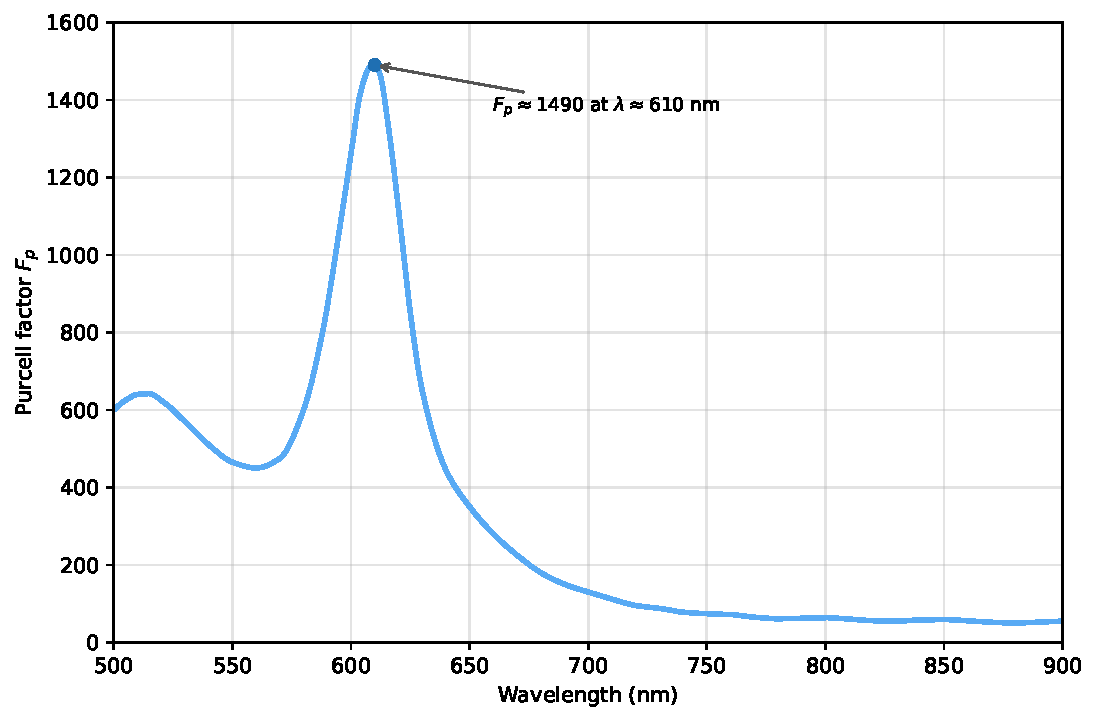
\includegraphics[width=0.88\linewidth]{figures/Test2_A_Purcell_full.pdf}
 \caption{طیف فاکتور پورسل حالت اصلی A برای نانومیله و دوقطبی طولی،
 رقم‌زنی و بازترسیم‌شده از تصویر خروجی Lumerical تست دوم. قله تقریبی
 $\Fp\simeq1490$ در حدود $\nm{610}$ قرار دارد.}
 \label{fig:purcell}
\end{figure}

\subsection{توان تابشی و موازنه انرژی}
\label{sec:results-radiated}

بیشینه تقویت توان تابشی حالت A برابر
$T_{\max}=119.219$ در حدود $\nm{616}$ به دست آمد
(شکل~\ref{fig:radiated}). قله تابشی تقریباً شش نانومتر سرخ‌تر از قله
پورسل است. این جدایی نشان می‌دهد که بیشینه کار انجام‌شده توسط چشمه و
بیشینه انرژی خارج‌شده از جعبه شار دقیقاً در یک طول‌موج رخ نمی‌دهند؛ جذب
اهمی طلا و وابستگی طیفی برون‌کوپل‌شدن میدان نزدیک در این تفاوت نقش دارند
\cite{bharadwaj2009optical}.

\begin{figure}[htbp]
 \centering
 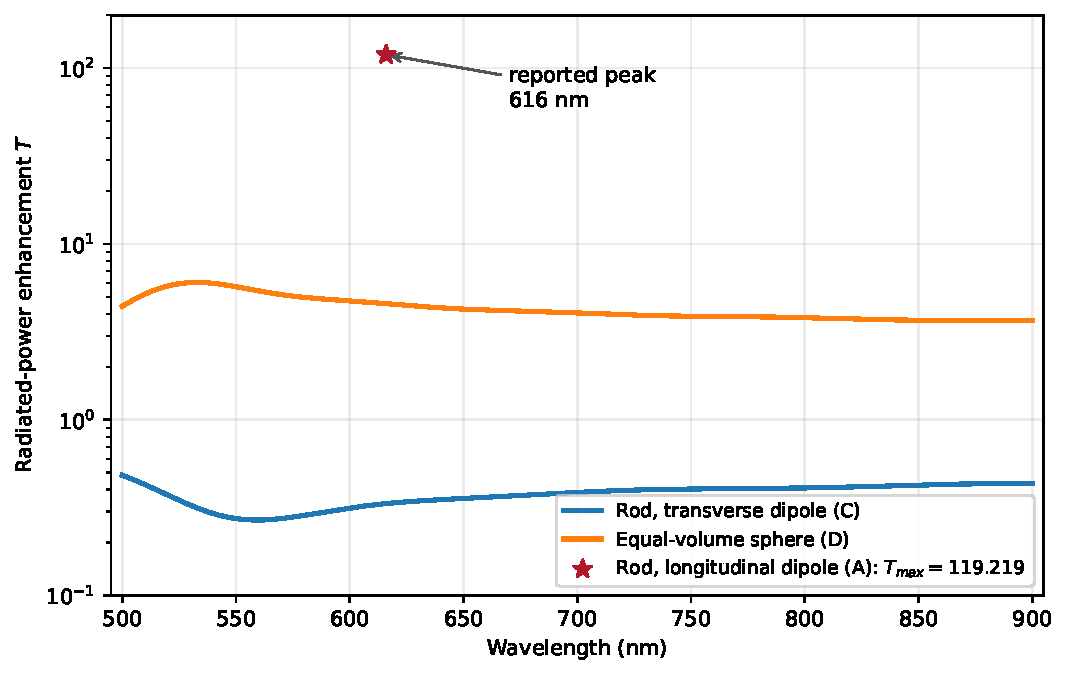
\includegraphics[width=0.88\linewidth]{figures/Test2_Radiated.pdf}
 \caption{تقویت توان تابشی تست دوم. ستاره قله گزارش‌شده حالت طولی A و
 منحنی‌ها خروجی کامل کنترل‌های C و D هستند. مقادیر هر سه حالت با تعریف
 خام $T=P_{\mathrm{rad}}/P_0$ رسم شده‌اند.}
 \label{fig:radiated}
\end{figure}

چون $\Fp$ و $T$ حالت A در دو طول‌موج متفاوت به بیشینه می‌رسند، تقسیم
مستقیم دو قله، راندمان طیفی دقیق نیست. بااین‌حال می‌توان یک کران معتبر
به دست آورد. در طول‌موج قله پورسل، توان تابشی نمی‌تواند از بیشینه کلی خود
بزرگ‌تر باشد؛ بنابراین
\begin{equation}
 \eta_a(\lambda_{F_p})=\frac{T(\lambda_{F_p})}{1490}
 \leq\frac{119.219}{1490}\simeq 8.0\%,
 \label{eq:eta-bound}
\end{equation}
و در نتیجه دست‌کم حدود ۹۲ درصد توان کل در آن طول‌موج وارد کانال‌های
غیرتابشی می‌شود. به‌طور مشابه،
\begin{equation}
 \frac{P_{\mathrm{loss}}(\lambda_{F_p})}{P_0}
 \geq1490-119.219=1370.781 .
 \label{eq:loss-bound}
\end{equation}
این بیان، برخلاف کم‌کردن دو قله در طول‌موج‌های متفاوت، یک کران فیزیکی
صحیح است و نتیجه اصلی یعنی غلبه خاموشی غیرتابشی در گپ پنج‌نانومتری را
حفظ می‌کند \cite{anger2006enhancement}.

\subsection{کنترل جهت‌گیری دوقطبی}
\label{sec:results-orientation}

حالت C اثر چرخاندن دوقطبی از راستای طولی به راستای عرضی را، بدون تغییر
هندسه و فاصله، اندازه می‌گیرد. قله خام آن
$F_p=239.235$ در $\nm{508}$ است، ولی توان تابشی در همان نقطه فقط
$T=0.4387$ و راندمان $0.183\%$ است. پس قله آبی C عمدتاً افزایش LDOS همراه
با جذب شدید است، نه یک تشدید تابشی کارآمد. پس از تصحیح با B، قله پورسل C
به $246.81$ در $\nm{506}$ می‌رسد.

در حوالی تشدید طولی، اختلاف بسیار بزرگ‌تر است. در $\nm{610}$ مقدار خام C
برابر $F_p=36.382$ است؛ بنابراین قله A تقریباً ۴۱ برابر بزرگ‌تر است. در
$\nm{616}$ نیز $T_C=0.3330$ است و بیشینه A حدود ۳۵۸ برابر آن است. این
کنترل مستقیم نشان می‌دهد پاسخ نانومیله یک کمیت همسانگرد نیست و جهت
دوقطبی باید صریحاً گزارش شود. بااین‌حال C کاملاً بدون جفت‌شدگی نیست؛ بیان
دقیق آن است که دوقطبی طولی با مد دوقطبی طولی نانومیله \emph{بسیار
مؤثرتر} از دوقطبی عرضی جفت می‌شود.

\subsection{کنترل کره هم‌حجم}
\label{sec:results-shape}

برای جداکردن اثر شکل از مقدار ماده، حالت D با کره‌ای به شعاع
$\nm{15.874}$ اجرا شد که حجمی برابر نانومیله دارد. قله خام کره
$F_p=658.738$ در $\nm{508}$ و قله تابشی آن $T=6.033$ در $\nm{532}$ است.
پس از تصحیح پایه، این دو قله به‌ترتیب $679.23$ و $6.063$ می‌شوند. در
$\nm{610}$ مقدار خام $F_p$ کره $96.131$ است؛ یعنی پاسخ طولی A تقریباً
۱۵٫۵ برابر بزرگ‌تر است. در $\nm{616}$ نیز $T_D=4.569$ و تقویت تابشی A
حدود ۲۶ برابر آن است. بنابراین تقویت نزدیک ۶۱۰ نانومتر صرفاً پیامد حجم
طلا نیست، بلکه به شکل کشیده و مد پلاسمونی طولی وابسته است. طیف کامل و
تصحیح‌شده کنترل‌های C و D در شکل~\ref{fig:cd-controls} آمده است.

\begin{figure}[htbp]
 \centering
 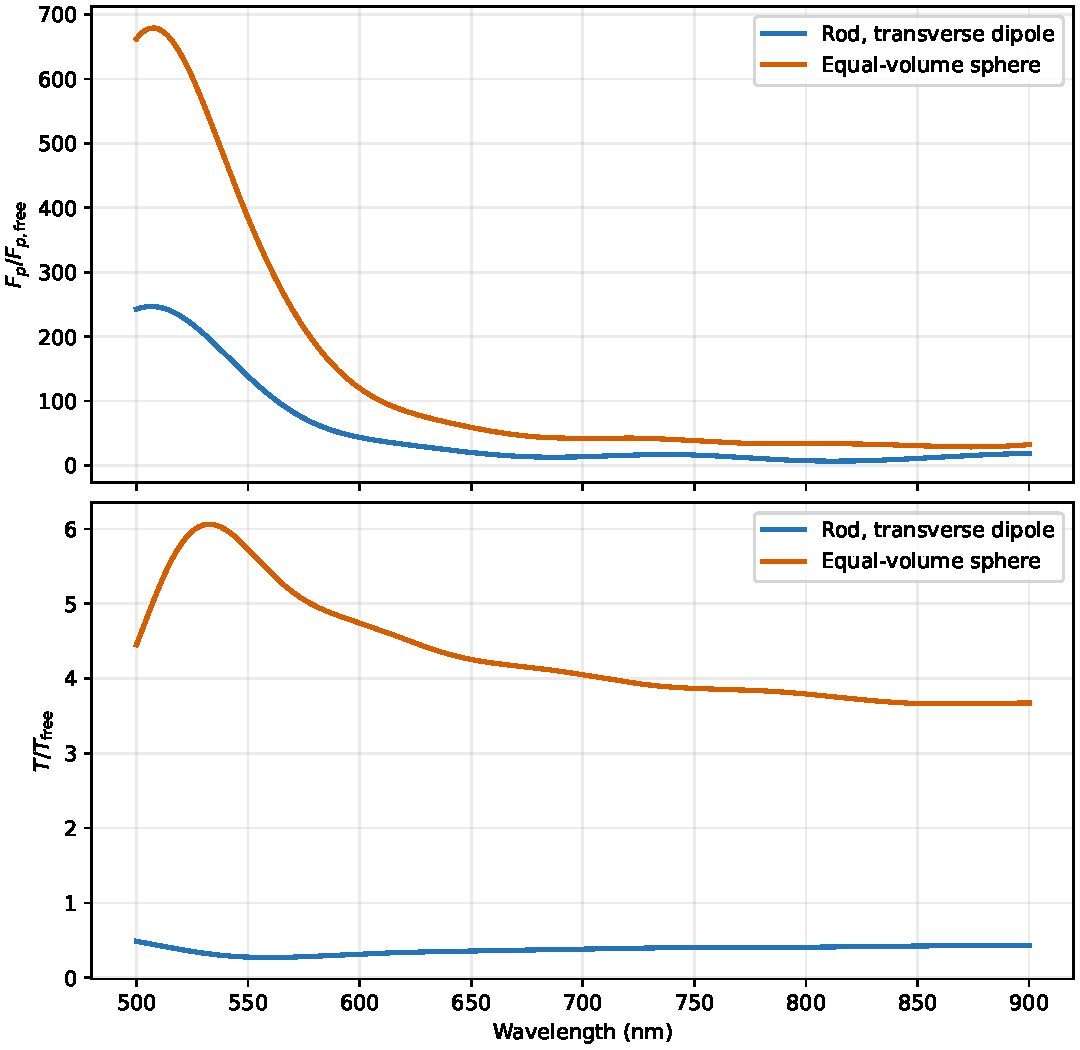
\includegraphics[width=0.92\linewidth]{figures/Test2_CD_Controls.pdf}
 \caption{طیف‌های تصحیح‌شده با مرجع فضای آزاد برای نانومیله با دوقطبی
 عرضی C و کره هم‌حجم D: فاکتور پورسل (بالا) و تقویت توان تابشی (پایین).
 این منحنی‌ها مستقیماً از فایل‌های ۲۰۱ نقطه‌ای Lumerical رسم شده‌اند.}
 \label{fig:cd-controls}
\end{figure}

\subsection{میدان نزدیک و محدودیت نمایش}
\label{sec:results-nearfield}

نقشه‌های میدان موجود C و D در شکل~\ref{fig:nearfield} با مقیاس لگاریتمی،
مرز هندسه و محل دوقطبی ترسیم شده‌اند. بیشینه C در
$(x,z)\simeq(0,\nm{35.08})$ و بیشینه D در
$(0,\nm{21.02})$ قرار دارد که با مکان چشمه‌ها سازگار است. میدان C در
$\nm{610}$ و میدان D در $\nm{530}$ ثبت شده‌اند؛ ازاین‌رو رنگ و مقدار
بیشینه دو پنل نباید به‌عنوان مقایسه مستقیم دامنه میدان تفسیر شود.

\begin{figure}[htbp]
 \centering
 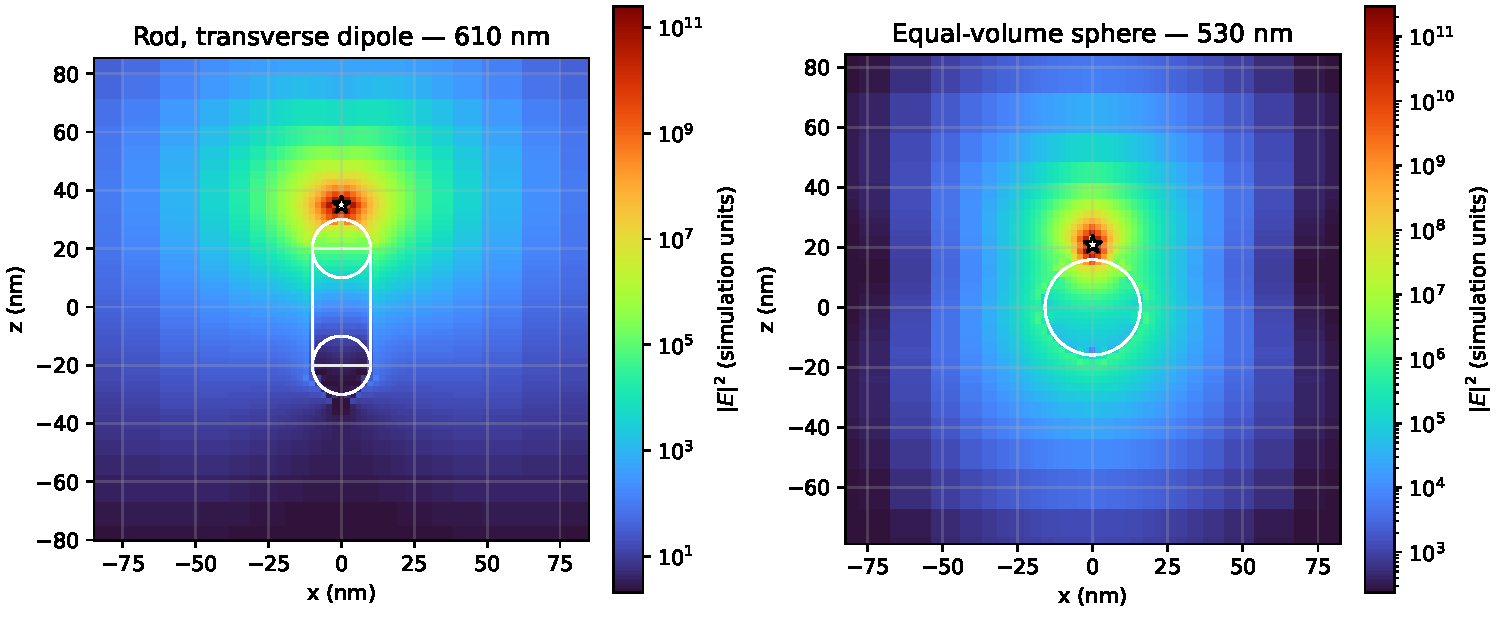
\includegraphics[width=0.98\linewidth]{figures/Test2_Nearfield_controls.pdf}
 \caption{نقشه لگاریتمی $|E|^2$ برای کنترل دوقطبی عرضی C در ۶۱۰ نانومتر
 (چپ) و کره هم‌حجم D در ۵۳۰ نانومتر (راست). خط سفید مرز فلز و ستاره محل
 دوقطبی است. طول‌موج و مقیاس رنگ دو پنل متفاوت‌اند.}
 \label{fig:nearfield}
\end{figure}

تمرکز بیشینه دقیقاً روی چشمه نقطه‌ای، بخشی از میدان نزدیک و تکین خود
دوقطبی است؛ بنابراین یک لکه روشن به‌تنهایی اثبات مود نیست. شناسایی مود
طولی در این پژوهش عمدتاً بر پاسخ طیفی A، اختلاف شدید A و C و مقایسه با
کره هم‌حجم تکیه دارد، نه فقط بر بیشینه یک پیکسل میدان.

\subsection{جمع‌بندی اعتبار عددی}
\label{sec:results-validity}

کنترل B برای T بسیار مطلوب است: $T_B$ در بازه ۵۰۰ تا ۹۰۰ نانومتر تقریباً
بین ۰٫۹۹۳ و ۱٫۰۰۳ باقی می‌ماند. در مقابل، $F_{p,B}$ مطابق
شکل~\ref{fig:free-baseline} تا ۱٫۱۳۳ تغییر می‌کند و وجود خطای پایه وابسته
به طول‌موج را نشان می‌دهد.

\begin{figure}[htbp]
 \centering
 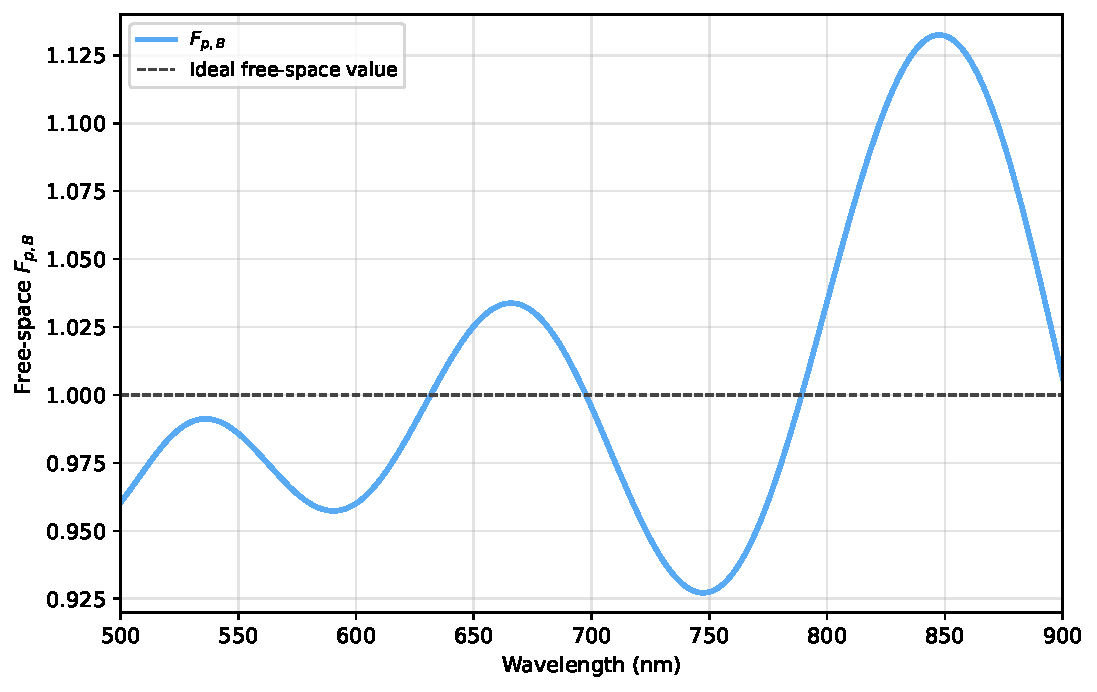
\includegraphics[width=0.84\linewidth]{figures/Test2_B_Freespace.pdf}
 \caption{خروجی فاکتور پورسل مرجع فضای آزاد B. خط‌چین مقدار ایده‌آل یک را
 نشان می‌دهد. انحراف طیفی از یک، عدم‌قطعیت عددی نرمال‌سازی را مشخص می‌کند.}
 \label{fig:free-baseline}
\end{figure}

این خطا نتیجه کیفی
مقایسه A، C و D را تغییر نمی‌دهد، ولی همراه با نبود آزمون همگرایی مش،
دقت اعداد قله را محدود می‌کند. ازاین‌رو اعداد تست دوم با تعداد رقم متناسب
گزارش شدند: مقدار پورسل A تقریبی، مقدار T مطابق خروجی موجود، و نتایج کامل
C و D با تصحیح طول‌موج‌به‌طول‌موج کنترل شدند. اجرای مش‌های ۳ و ۱٫۵
نانومتر و گپ‌های دیگر در اسکریپت تعریف شده، ولی در مجموعه حاضر اجرا نشده
است و به‌عنوان کار آینده باقی می‌ماند.

% ===================================================================
%  بخش ۵ — نتیجه‌گیری  (بازنویسی بر پایه‌ی اجرای دوم)
% ===================================================================
\section{نتیجه‌گیری}
\label{sec:conclusion}

در این پژوهش، پاسخ یک گسیل‌گر دوقطبی در فاصله‌ی پنج نانومتری از نانومیله‌ی
طلای کلاهک‌دار با روش 3D-FDTD در ده اجرای کنترل‌شده و اسکریپت‌محور
بررسی شد (جدول~\ref{tab:cases}: A, B, C, D, D$_\perp$, M3, M1.5, G3, G10, G20). برای دوقطبی طولی، فاکتور پورسل در $\nm{610}$ به $1.5\times10^{3}$
و تقویت توان تابشی در $\nm{616}$ به $1.2\times10^{2}$ می‌رسد. طیف کامل
بازده نشان می‌دهد که در قله‌ی پورسل تنها $7.6\%$ و در قله‌ی تابشی
$8.6\%$ توان تابیده می‌شود و بیش از $92\%$ به کانال غیرتابشی می‌رود؛
گزارش فاکتور پورسل به‌تنهایی برای ارزیابی نانوآنتن کافی نیست.

چهار کنترل نقش جهت و شکل را از هم جدا کردند. چرخاندن دوقطبی به راستای
عرضی روی همان نوک، فاکتور پورسل در تشدید را $41$ برابر و توان تابشی را
$360$ برابر کاهش داد. اما نتیجه‌ی تعیین‌کننده از مقایسه با کره‌ی هم‌حجم
با دو جهت‌گیری شعاعی و مماسی به دست آمد: نسبت جهتی کره در کل طیف
تقریباً ثابت و نزدیک $2.4$ است، و نسبت جهتی نانومیله در خارج از تشدید
دقیقاً همین مقدار است ولی در تشدید طولی یک تا دو مرتبه‌ی بزرگی می‌جهد.
بنابراین ناهمسانگردی تانسور گرین نانومیله دو سهم دارد: سهم هندسی
نزدیک‌سطحی از مرتبه‌ی $2$ که هر جسم فلزی دارد، و سهم تشدیدی که تنها به
مد طولی محور ممتاز تعلق دارد و توصیف اسکالر یا میانگین‌گیری جهتی آن را
حذف می‌کند. پویش گاف نیز نشان داد که با افزایش گاف از $5$ به $\nm{20}$
مکان تشدید ثابت می‌ماند، قله‌ی تابشی از $119$ به $10$ می‌افتد و بیشینه‌ی
بازده طیفی از $19\%$ به $74\%$ می‌رسد.

اعتبار عددی با سه آزمون سنجیده شد. کنترل فضای آزاد صحت شار را تأیید کرد
ولی حساسیت $\pm13\%$ نرمال‌سازی را نشان داد؛ مقایسه با حل می برای کره،
مکان قله‌ها را با اختلاف $\nm{2}$ بازتولید و کم‌برآوردی $8$ تا $14\%$
مش $\nm{2}$ را کمّی کرد؛ و آزمون همگرایی مش ($3$، $2$ و $\nm{1.5}$)
آشکار ساخت که مکان قله‌ی تابشی ($616\pm\nm{4}$) و بازده در آن پایدارند،
ولی ارتفاع قله‌ها به دلیل قرارگیری زیرسلولی چشمه در گاف پنج‌نانومتری
تا $\pm40\%$ تغییر می‌کند. به همین دلیل، ادعاهای این مقاله آگاهانه بر
مکان تشدیدها، بازده و نسبت‌های میان حالت‌های هم‌مش استوار شده‌اند و
ارتفاع مطلق قله‌ها با این عدم‌قطعیت گزارش می‌شود.

دامنه‌ی ادعای مقاله محدود به همین سامانه‌ی کلاسیک و موضعی است. نتایج به
معنی نامعتبر بودن ضرایب اینشتین برای اتم آزاد یا نظریه‌ی می برای کره
نیستند؛ بلکه نشان می‌دهند در محیط ناهمسانگرد و اتلافی، نرخ کل، نرخ تابشی
و جهت‌گیری دوقطبی باید جداگانه مشخص شوند. گام بعدی روشن و مشخص است:
اجرای حالت اصلی با مش $\le\nm{1}$ و چشمه‌ی دقیقاً روی گره (یا مش
ناهمسانگرد ریز در راستای گاف) تا ارتفاع قله‌ها نیز همگرا شود؛ اجرای
مرجع فضای آزاد با همان مش و مختصات؛ و گزارش برازش داده‌ی طلا. توسعه‌ی
پایه‌ی مدی متناسب با تقارن استوانه‌ای
\cite[pp.~123--131]{maier2007plasmonics} و بررسی پاسخ غیرموضعی موضوع
کار آینده‌اند.

از دید کاربردی، تقویت بیش از صدبرابری توان تابشی نشان می‌دهد نانومیله‌ی
طلا برای کاربردهایی که نرخ گسیل و شدت سیگنال مهم‌تر از بازده‌اند —
حسگری فلورسانسی و طیف‌سنجی تقویت‌شده — مفید است؛ اما برای چشمه‌ی
تک‌فوتونی، که به بازده جمع‌آوری بالا نیاز دارد، پویش گاف حاضر
(شکل~\ref{fig:gap}) نشان می‌دهد گاف $10$ تا $\nm{20}$ با تقویت تابشی
$10$ تا $50$ برابری و بازده رو به بهبود، مصالحه‌ی معقول‌تری است
\cite{mohammadi2008gold, koenderink2017single}. تحقق تجربی چنین
ساختاری نیز به کنترل اندازه و شکل نانومیله در فرآیند سنتز وابسته است
\cite{nikoobakht2003preparation}.

% ===================================================================
%  پیوست الف — فهرست نمادها و اختصارها
%  هدف: یک‌جا آوردن همه‌ی نمادهای پرکاربرد تا خواننده (به‌ویژه در
%  ارائه‌ی کلاسی) بدون گشتن در متن، معنا و یکای هر کمیت را ببیند.
%  اعداد و تعریف‌ها با بخش‌های ۳ و ۴ هم‌خوان‌اند.
% ===================================================================
\appendix
\section*{پیوست الف: فهرست نمادها و اختصارها}
\label{sec:appendix-nomenclature}
\addcontentsline{toc}{section}{پیوست الف: فهرست نمادها و اختصارها}

جدول~\ref{tab:nomenclature} نمادها و اختصارهای پرکاربرد این مقاله را یک‌جا
گرد آورده است. سه کمیت نخست ($\Fp$، $T$ و $\eta_a$) سه ستون فقرات تحلیل
این پژوهش‌اند: نرخ واپاشی کل، کانال تابشی و نسبت میان آن دو.

\begin{table}[htbp]
  \centering
  \caption{فهرست نمادها و اختصارهای پرکاربرد.}
  \label{tab:nomenclature}
  \begin{tabular}{lll}
    \toprule
    نماد / اختصار & معنا & یکا / توضیح \\
    \midrule
    $\Fp$ & فاکتور پورسل: نسبت نرخ واپاشی کل به نرخ در فضای آزاد
          & بی‌بعد (رابطه~\eqref{eq:Fp}) \\
    $T$ & ضریب تقویت توان تابشی میدان دور
          & بی‌بعد (رابطه~\eqref{eq:T}) \\
    $\eta_a$ & بازده کوانتومی ظاهری، $\eta_a = T/\Fp$
          & بی‌بعد، گزارش‌شده به درصد \\
    $P_0$ & توان گسیل‌شده‌ی دوقطبی در فضای همگن & وات \\
    $P_{\text{rad}}$ & توان تابش‌شده به میدان دوردست & وات \\
    $P_{\text{loss}}$ & توان اتلافی غیرتابشی (اهمی) در فلز & وات \\
    $\Gamma_{\text{tot}}$، $\Gamma_0$ & نرخ واپاشی کل / نرخ در فضای همگن
          & $\text{s}^{-1}$ \\
    $\lambda_{\text{res}}$ & طول‌موج قله‌ی فاکتور پورسل & $\nm{607.9}$ در این کار \\
    $\lambda_{\text{rad}}$ & طول‌موج قله‌ی توان تابشی & $\nm{615.1}$ در این کار \\
    $L$، $D$، $R$ & طول کل، قطر و شعاع کلاهک نانومیله & $\nm{60}$، $\nm{20}$، $\nm{10}$ \\
    $d$ & فاصله‌ی دوقطبی تا راس کلاهک & $\nm{5}$ \\
    $l$، $m$ & مرتبه‌ی چندقطبی کروی و شماره‌ی آزیموتالی & بی‌بعد \\
    $\beta$ & ثابت انتشار محوری در هندسه‌ی استوانه‌ای & $\text{rad/m}$ \\
    \midrule
    LDOS & چگالی موضعی حالات فوتونی & --- \\
    LSPR & پلاسمون سطحی موضعی & --- \\
    FDTD & تفاضل محدود در حوزه زمان & --- \\
    PML & لایه‌ی جاذب کاملاً منطبق (مرز محاسباتی) & --- \\
    QNM & مد شبه‌نرمال (مدهای کاواک با فرکانس مختلط) & --- \\
    \bottomrule
  \end{tabular}
\end{table}


% ===================================================================
\printbibliography[title={مراجع}]

\end{document}
